\documentclass[9pt,twocolumn,twoside]{opticajnl}
\journal{opticajournal}

\setboolean{shortarticle}{true}

\usepackage{lineno}

\title{Finite-size--corrected synchronization in a city-scale bus network:
crossover, not criticality}

\author[1,*]{Po-Hsun, Lai}


\affil[1]{Physics, National Taiwan University, Taipei, Taiwan}


\affil[*]{b11202025@ntu.edu.tw}

\setboolean{displaycopyright}{false}

%% ----------------------------------------------------------------------
%% FIGURE FILES (from the analysis output tree). Copy these next to the .tex
%% or compile from the project root using the \graphicspath below.
%%   Fig 1 : outputs/phase4/figures/p4_5_synthesis.pdf
%%   Fig 2 : outputs/phase4/figures/p4_3_amplification_drivers.pdf
%%   Fig 3 : outputs/phase4/figures/p4_1_corridor_speed_gate.pdf
%% ----------------------------------------------------------------------
\graphicspath{{../Figure/}{./}}

\begin{abstract}
Bus bunching is widely read as phase synchronization of coupled oscillators, with sustained
clustering emerging once passenger demand exceeds a threshold. Testing that picture on real
networks requires a synchronization observable that is comparable across time and place ---
and we show that the natural one is not. On 13.8M GPS fixes and 6.8M boardings from the
NetMob26 Niter\'oi dataset, the raw Kuramoto order parameter is severely confounded by the
number of buses in a cell: small fleets read as synchronized for purely statistical reasons.
Correcting against a same-$N$ random-phase null reverses a substantive conclusion --- weekends,
which look more synchronized in the raw signal, are in fact less synchronized --- and recasts
the demand dependence as a smooth crossover rather than a sharp critical transition (one of
three pre-registered criticality signatures passes). Downstream headway amplification is more
strongly associated with inherited upstream irregularity than with realized load, and the
co-synchronization of lines on a shared trunk is largely consistent with shared road-state
exposure once segment speed is controlled. What reads as collective synchronization in raw
transit data is, here, a mixture of finite-size bias, operational dispatch irregularity, and
common road-state shocks. Finite-size null correction is a prerequisite for interpreting
field synchronization observables as collective dynamics.
\end{abstract}

\begin{document}

\maketitle

\section{Problem and data}
A bus that falls behind schedule meets more waiting passengers, dwells longer, and falls
further behind, until the following bus catches it: the headways collapse and buses bunch.
Newell and Potts framed this instability in 1964 \cite{newell64}, and a complex-systems
reading treats each line as a ring of coupled self-oscillators whose phases lock under load,
in analogy with the Kuramoto transition \cite{saw19,strogatz00}. That analogy predicts a
demand-driven onset of collective synchronization. It has been examined almost entirely in
simulation or on single shuttle loops; a city-scale, multi-line test with fused vehicle
telemetry and passenger demand has been missing, largely for want of such data
\cite{schlapfer21}.

The NetMob26 dataset \cite{netmob26} supplies it for Niter\'oi, Brazil. We use 19 days of
telemetry (11--31 March 2026; 13{,}850{,}467 GPS fixes from 527 vehicles at 15--30\,s
spacing) and the full ticketing feed (6{,}790{,}681 boardings). The two feeds carry no common
vehicle key, which fixes the identification scope of the study: passenger exposure is defined
at the \textit{line--direction--hour} level, and every demand-related quantity below is
cell-level rather than vehicle-level. This is the unit at which supply and demand can be
aligned in these data, and we treat it as the analysis unit by design.

\section{Synchronization observable}
For each of 20 high-ridership lines we project GPS onto the route polyline
(\texttt{line\_routes.json}, with GTFS \texttt{shapes.txt} as fallback), reduce position to
arc length $s$, and assign a phase $\varphi = 2\pi s / L$ per direction, so the buses on a
\textit{(line, direction, hour)} cell become oscillators on a ring. After dropping routes that
fail map-matching and excluding terminal-layover and sparsely sampled bus-hours
(69{,}466 active bus-hours retained), we compute the first Kuramoto--Daido order parameter
\begin{equation}
r_1 = \Big| \tfrac{1}{N}\sum_{j=1}^{N} e^{i\varphi_j} \Big|,
\label{eq:r1}
\end{equation}
near $0$ for evenly spread buses (the splay state) and near $1$ when they bunch.

The order parameter is not comparable across cells. For $N$ uniformly random phases
$\mathbb{E}[r_1]\approx 0.886/\sqrt{N}$, so a cell with few buses reports a high $r_1$ with no
underlying coordination, and any quantity that covaries with fleet size --- weekends, off-peak
hours, low-demand lines --- inherits a spurious synchronization signal. We therefore draw
5{,}000 random-phase samples at each observed $N$ and report a finite-size--corrected
synchronization,
\begin{equation}
r_{\mathrm{exc}} = \frac{r_1 - \mathbb{E}_{\mathrm{null}}[r_1\,|\,N]}{1 - \mathbb{E}_{\mathrm{null}}[r_1\,|\,N]},
\qquad
z = \frac{r_1 - \mathbb{E}_{\mathrm{null}}[r_1\,|\,N]}{\mathrm{sd}_{\mathrm{null}}[r_1\,|\,N]} ,
\label{eq:rexc}
\end{equation}
which measure how far a cell sits above its same-$N$ random baseline. This correction is the
central methodological contribution of the paper: in a transit system with fluctuating fleet
sizes it is a prerequisite for any field measurement of synchronization, and every value
below is reported with its $N$.

\begin{figure*}[t]
\centering
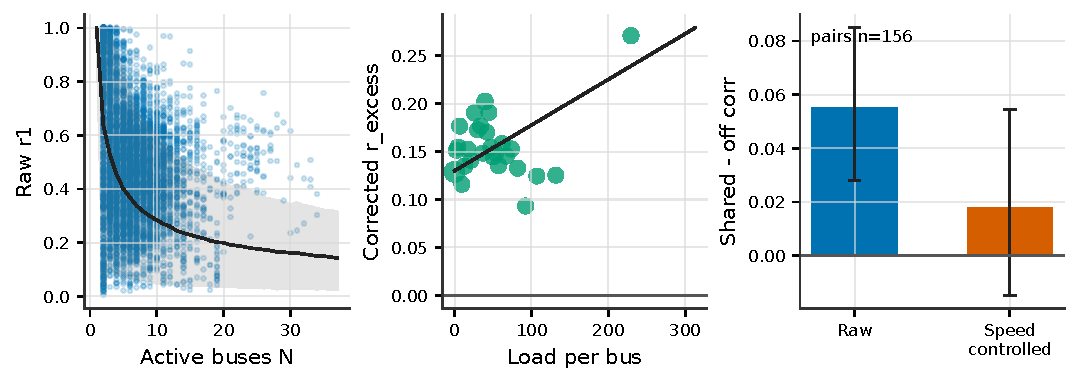
\includegraphics[width=\textwidth]{p4_5_synthesis.pdf}
\caption{The argument in one figure. Raw $r_1$ is finite-size confounded, tracking the active
fleet size rather than coordination; correcting against a same-$N$ random-phase null reverses
the apparent weekend effect (weekends are \emph{less} synchronized once corrected); the
dependence of corrected synchronization on realized load per bus $\lambda$ is a smooth
crossover, with no sharp onset; and the cross-line signal on shared corridors attenuates
toward zero once the common road state (segment speed) is controlled. Panels reproduced from
the Phase~4 synthesis output.}
\label{fig:syn}
\end{figure*}

\section{Results}

\paragraph{Result 1 --- finite-size correction reverses the apparent weekend effect.}
In the raw signal weekends look \emph{more} synchronized than weekdays
(weekend$-$weekday $r_1 = +0.047$, 95\% CI $[0.039,0.056]$), despite running far fewer buses.
This is exactly the regime where $r_1$ is least trustworthy, and the correction overturns it:
weekend$-$weekday $r_{\mathrm{exc}} = -0.067$ ($[-0.085,-0.048]$) and $z = -0.441$
($[-0.486,-0.397]$); corrected synchronization is \emph{lower} on weekends
(Table~\ref{tab:cmp}). The reversal is not a cosmetic adjustment --- it changes the substantive
conclusion about when the system is most coordinated --- and it is the clearest empirical
demonstration that raw Kuramoto observables cannot be compared across cells of different $N$.

\paragraph{Result 2 --- demand modulates synchronization, but without a sharp transition.}
We summarize cell-level load as $\lambda = \text{boardings}/N$. Because $N$ is itself an
operational response to demand and conditions, $\lambda$ should be read as realized load per
active bus, not exogenous passenger demand. Corrected synchronization rises with $\lambda$
(standardized random-intercept coefficient $0.039$, $p\approx 3\times10^{-15}$), and a
piecewise fit places an apparent break at $\lambda \approx 136$ boardings/bus. We treat this
as an observational crossover scale, not a critical point, because a pre-registered three-part
gate does not support criticality. The susceptibility check asks whether fluctuations in
$r_{\mathrm{exc}}$ peak at an interior $\lambda$ (the signature of a transition); within
$N$-strata they do not (peak/edge ratios $0.89$--$1.14$). The coexistence check asks whether
low- and high-synchronization states co-occur near the candidate scale; the order-parameter
distribution is no more bimodal there than elsewhere ($\Delta\mathrm{BIC}\approx 18$, weaker
than off-scale regimes). The $N$-stability check asks whether the apparent scale is more than
fleet-size composition; this one passes. With one of three signatures met, the honest reading
is a smooth, demand-modulated crossover rather than city-scale criticality.

\paragraph{Result 3 --- mechanisms are operational and common-shock dominated.}
We examined two routes by which a genuine oscillator-coupling story might persist, and both
resolve toward operational explanations. \emph{Downstream amplification.} Headway irregularity
grows along the route interior (mean headway-CV slope $0.12$, $p\approx 2\times10^{-58}$ on
the 10--90\% interior), the spatial fingerprint of the Newell--Potts instability. In a
standardized model (Fig.~\ref{fig:drivers}) this growth is more strongly associated with the
irregularity already inherited upstream ($-0.283$, $[-0.296,-0.270]$) than with contemporaneous
realized load ($0.015$, $[0.002,0.027]$) or fleet size ($0.081$), with route topology
unresolved; the negative sign on the upstream term reflects a ceiling --- already-irregular
hours have less room to grow downstream --- not a stabilizing effect of irregularity.
\emph{Dwell mediation.} The classic $\lambda \to$ dwell-time variability $\to$ bunching channel
is not established in these data (indirect effect $\approx 0.0001$, proportion mediated
$0.2\%$), partly because boardings are not linked to individual vehicles and GPS-derived dwell
is noisy; we do not read this as ruling the mechanism out. \emph{Shared corridors.} Lines on a
common trunk are more co-synchronized on the shared segment than off it (within-pair raw gap
$0.055$, $[0.028,0.085]$; 156 pairs). Controlling for the shared-segment mean bus speed --- the
common road state --- the gap falls to $0.018$ ($[-0.015,0.054]$), retaining about a third and
now spanning zero, and lead--lag and transfer-entropy tests show no propagation (5.8\% of pairs
with a non-zero-lag peak; net directional asymmetry $p=0.87$; Fig.~\ref{fig:syn}, right panel). The
co-synchronization is largely consistent with shared road-state exposure; a residual inter-line
coupling is not established, though speed control may also absorb part of a genuine coupling
channel.

\begin{table}[t]
\centering
\caption{\bf Corrected synchronization by day type and period$^{a}$}
\begin{tabular}{lccccc}
\hline
Group & $N$ & $r_1$ & $r_{\mathrm{exc}}$ & $z$ & $\lambda$ \\
\hline
Weekday            & 7.99  & 0.482 & 0.179 & 0.806 & 57.6 \\
Weekend            & 4.47  & 0.529 & 0.112 & 0.366 & 40.3 \\
Weekday, off-peak  & 7.23  & 0.499 & 0.178 & 0.758 & 63.7 \\
Weekday, peak      & 10.82 & 0.420 & 0.180 & 0.985 & 34.7 \\
Weekend, off-peak  & 4.34  & 0.537 & 0.113 & 0.356 & 41.2 \\
Weekend, peak      & 4.95  & 0.504 & 0.109 & 0.400 & 37.3 \\
\hline
\end{tabular}
\label{tab:cmp}

\smallskip
$^{a}$Raw $r_1$ is higher on weekends; finite-size--corrected $r_{\mathrm{exc}}$ and $z$ are
lower. $\lambda$ is realized boardings per active bus.
\end{table}

\begin{figure}[t]
\centering
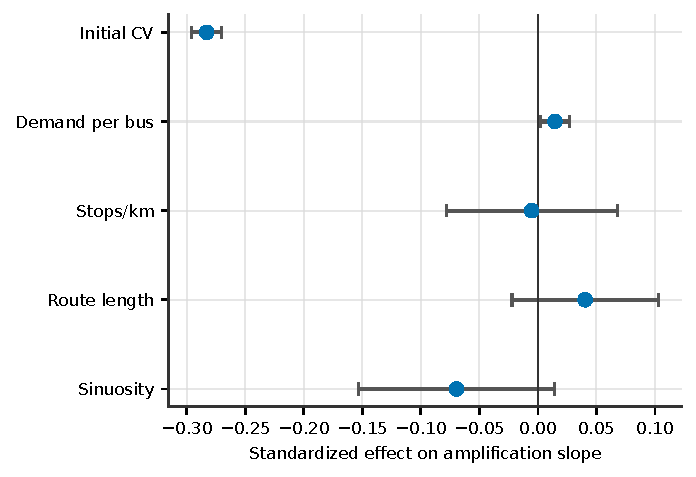
\includegraphics[width=\linewidth]{p4_3_amplification_drivers.pdf}
\caption{Inherited upstream irregularity, not realized load, is the strongest predictor of
downstream headway-CV growth. Standardized effects from a line--direction random-intercept
model with 95\% CIs; the negative upstream-irregularity coefficient is a ceiling effect. Realized load per bus is small
and route topology is unresolved.}
\label{fig:drivers}
\end{figure}

\section{Conclusion}
What appears as collective synchronization in raw transit data can be a mixture of finite-size
bias, operational dispatch irregularity, and common road-state shocks. In Niter\'oi, once the
order parameter is corrected against its same-$N$ random baseline, the demand dependence is a
smooth crossover rather than a critical transition; downstream amplification tracks inherited
irregularity more than realized load; and shared-corridor co-synchronization is largely a
shared road state. The methodological point generalizes: empirical synchronization observables
must be corrected against finite-size null models before they are interpreted as collective
dynamics or critical phenomena, in transit and in other finite, fluctuating ensembles measured
in the field. Two steps would sharpen identification further --- a propagation-aware coupling
model able to separate inter-line transfer from shared road shocks, and vehicle-linked
boarding data with a cleaner dwell signal to test the demand mechanism directly.

\begin{thebibliography}{9}
\bibitem{newell64} G.~F. Newell and R.~B. Potts, in \emph{Proc. 2nd ARRB Conf.} (1964), pp. 388--393.
\bibitem{saw19} V.-L. Saw, L.~Vismara, and L.~Y. Chew, Sci. Rep. \textbf{9}, 6887 (2019).
\bibitem{strogatz00} S.~H. Strogatz, Physica D \textbf{143}, 1 (2000).
\bibitem{schlapfer21} M.~Schl\"apfer, L.~Dong, K.~O'Keeffe, \emph{et al.}, Nature \textbf{593}, 522 (2021).
\bibitem{netmob26} F.~Domingos, H.~T. Marques-Neto, B.~Pereira, \emph{et al.}, arXiv:2605.20263 (2026).
\bibitem{kuramoto75} Y.~Kuramoto, in \emph{Int. Symp. Math. Problems in Theor. Phys.}, Lect. Notes Phys. \textbf{39} (1975), p. 420.
\end{thebibliography}

\end{document}
